% Slide 3 | Model and E2a | M4 (Vismay Shanbhag) | 2:00 | ADF test and its power
\begin{frame}{The ADF test, and what one year of data can detect}
\framesubtitle{Slide 3 \textbullet\ Model and E2a \textbullet\ M4 \textbullet\ 2:00}
\vspace{-2pt}
\begin{columns}[T,onlytextwidth]
\column{0.47\textwidth}
  \small\raggedright
  \textbf{\color{deckAccent}The regression}
  {\footnotesize\[ \Delta X_t=a+\gamma X_{t-1}+\sum_{i=1}^{p}\delta_i\,\Delta X_{t-i}+\varepsilon_t \]
  \[ \gamma=e^{-\kappa\Delta}-1 \]}
  \begin{itemize}\setlength{\itemsep}{2pt}
    \item $H_0:\gamma=0$ means $\kappa=0$, a random walk
    \item lagged differences clean the noise; lags chosen by AIC
    \item 5\% critical value $-2.86$, not $-1.65$
  \end{itemize}
\column{0.50\textwidth}
  \centering
  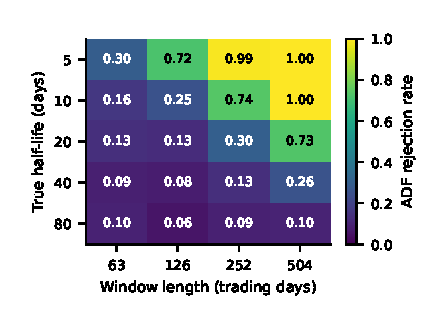
\includegraphics[width=\linewidth]{fig_e2_adf_power_report}\\[2pt]
  \footnotesize\raggedright
  \textbf{E2a:} ADF finds a gap that really closes \textbf{99\%} of the time at a 5-day half-life, \textbf{74\%} at 10 days, \textbf{30\%} at 20 days
\end{columns}
\pairTakeaway{One year only sees fast pairs: every pair we select has a half-life of 15 days or less.}
\end{frame}
